\section{Theoretical Analysis with River Valley Loss Landscapes}
\label{sec:optimization}

\begin{wrapfigure}{r}{0.32\textwidth}
    \centering
    \vspace{-0.2in}
    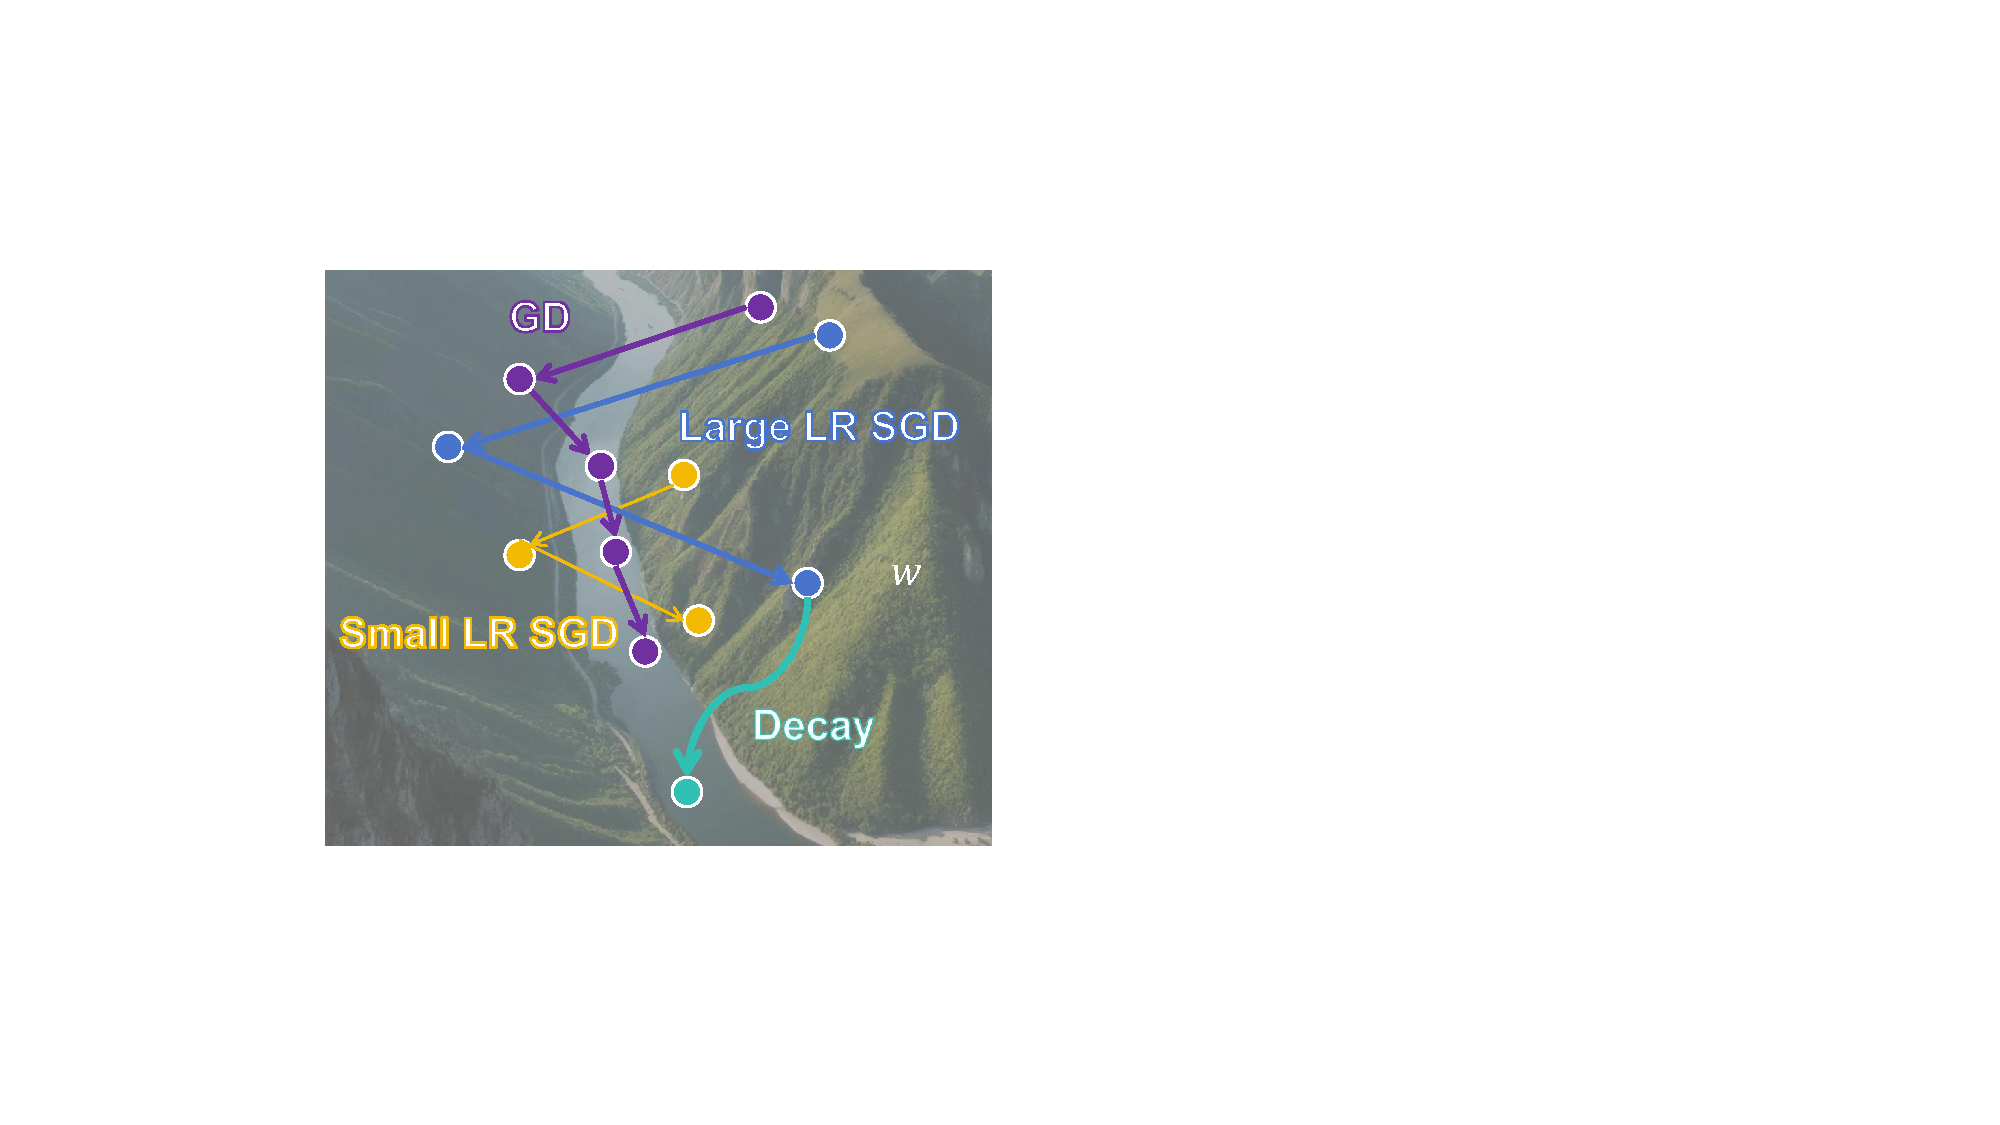
\includegraphics[width=0.3\textwidth]{figures/arxiv/function2.pdf}
    \caption{A River Valley Loss Landscape and the Optimization Dynamics with Various Learning Rates.}
    \label{fig:demo}
    \vspace{-0.2in}
\end{wrapfigure}

\textbf{Intuition and Outline.} As illustrated in Figure \ref{fig:demo}, we will analyze the dynamics of different optimization algorithm on the river valley loss landscape. (1) The \textcolor{purple}{gradient descent (GD)} iterates will quickly converge to the river and track the river afterward (\Cref{thm:gdtracksriver}). This holds for the continuous limit of GD, gradient flow, as well (\Cref{thm:gftracksriver}). (2) Stochastic gradient descent (SGD) algorithm on a river valley loss landscape will bounce between the hillsides due to the noise instead of converging to the river, while still gradually progressing along the river over time (\Cref{thm:sgd-main}). A 
large learning rate results in significant oscillations but also facilitates rapid advancement in the river's direction (the \textcolor{blue}{blue} trajectory). Conversely, a small learning rate keeps the iterates closer to the river's course but leads to slower movement along it (the \textcolor{darkyellow}{yellow} trajectory). While the oscillations in the mountain direction can cause a higher loss for a large learning rate in the short term, the large learning rate leads to faster fundamental progress along the river.
(3) Finally, reducing the learning rate before termination (the \textcolor{microsoftcyan}{cyan} trajectory) helps mitigate these oscillations and reveal the underlying fundamental progress in the river's direction (\Cref{thm:decay-main}). In this scenario, the $\wsd$ algorithm is preferred: the stable phase allows for substantial progress along the river, and the final decay phase reduces oscillations, ensuring that the iterates terminate near the river's course.



\subsection{Setting and Assumptions}

We will now formally present our theory. We use $w \in \R^d$ to denote the parameters and $L$ to denote the loss. Further, we use $\eigen{k}{H}$ and $\eigenv{k}{H}$ to denote the $k$-th largest eigenvalue and eigenvector of a matrix $H$, respectively. The ``river'' in the river valley is a 1-dimensional manifold $\river$ formalized below.

\begin{assumption}
\label{assum:river}
    We assume the existence of a ``river'', which is a 1-dimensional manifold $\river$ such that any point $w \in \river$ has a gradient $\nabla L(w)$ that is in the same direction as the minimal eigenvector direction of the Hessian, $\eigenv{d}{\nabla^2 L(w)}$. 
\end{assumption}
\begin{wrapfigure}{r}{0.3\textwidth}
    \centering
    \vspace{-0.5in}
    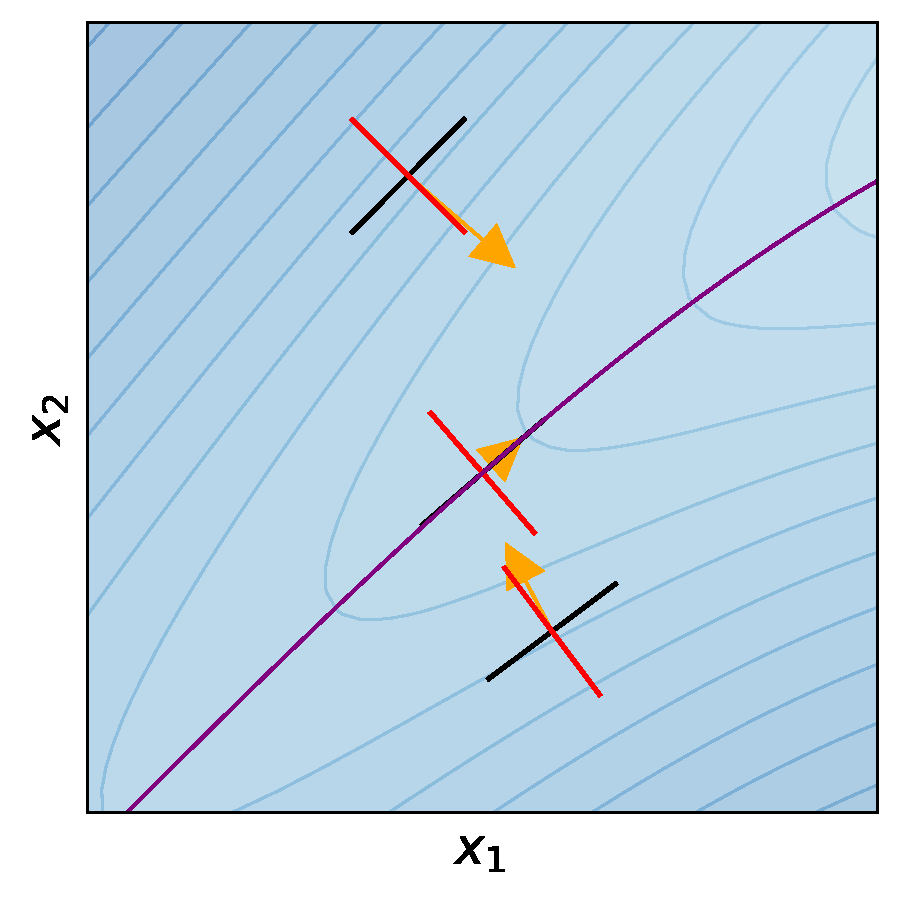
\includegraphics[width=0.3\textwidth]{figures/arxiv/eigenvectors_gradient.pdf}
    \caption{Illustration of the Definition of the River.}
    \label{fig:river}
    \vspace{-0.9in}
\end{wrapfigure}
Under this assumption, at every point on the river, the gradient $\nabla L(w)$ will align with the locally flattest direction, $\eigenv{d}{\nabla^2 L(w)}$, which we refer to as the \emph{river direction}. All other directions orthogonal to the river direction are considered as the \emph{mountain directions}, corresponding to the steep hillsides in our conceptual picture.
This definition is illustrated in the 2-dimensional loss landscape shown in \Cref{fig:river}. In this figure, the {\color{red}red} line represents the top eigenvector (the sharpest direction), while the black line represents the smallest eigenvector (the flattest direction) at each point. Along the \textcolor{blue}{blue} curve, which represents the river, the {\color{orange}orange} negative gradient aligns with the river direction.
For a point on the hillside, the negative gradient pulls the point downward along the hillside towards the river, while also while also moving it along the river. This intuition will be rigorously formalized in the theorems that follow.




To analyze the optimization dynamics, we will consider a neighborhood $U$ of the river $\river$. Inside this neighborhood, we will impose several technical assumptions. For example, we will assume that the Hessian has an eigengap between the smallest and the second smallest eigenvalues, so that the river direction is well-defined in $U$. We will also assume that the last eigenvector of the Hessian $v_d$ changes slowly, which implies that the river direction does not change rapidly during optimization. We summarize these assumptions below.

\begin{assumption}[Regularity Assumption]
\label{assum:technical}
    There exists an open set $U$ containing $\river$ satisfying the following assumptions:
    \begin{enumerate}[leftmargin=*]
        \item {Analyticity.} $L(w)$ is analytic with respect to $w$.
        \item {Bounded Hessian.}  There exists a constant $\maxgamma > 0$, such that $\forall w \in U, \| \nabla^2 L(w) \|_{\textup{op}} \le \maxgamma.$
        \item {Existence of Eigengap.} There exist constants $\flatgamma, \gamma > 0$, such that $$\forall w \in U, \eigen{d - 1}{\nabla^2 L(w)} > \gamma + 4 \flatgamma, |\eigen{d}{\nabla^2 L(w)}| < \flatgamma.$$
            \vspace{-0.2in}
        \item  {Slow Spinning of $v_d$.} There exist constants $\normbound > 0, \err \in [0, 0.01)$, such that $$\forall w \in U, \normbound_{\min} < \| \nabla L(w) \|_2 \le \normbound, \textup{ and } \| \nabla  \eigenv{d}{ \nabla^2 L(w)} \|_{\textup{op}}  \le \err \gamma/(2\normbound).$$
        This means that the river direction $v_d$ changes slowly during optimization.
        \item {Uniqueness of $\river$.} For any point $w \in U - \river$, the gradient $\nabla L(w)$ is not parallel to $v_d(\nabla^2 L(w))$.
        \item {Conservation of Gradient Flows.} There exists an open subset $V \subset U$ and  a constant $r > \frac{10 \normbound}{\gamma}$ for $\gamma$ defined in Assumption 2.3 such that $\forall w \in V$, the $r$-neighborhood of the gradient flow starting from $w$ stays in $U$ for continuous time $\maxT \ge {10 \log(2 \normbound / (\err \normbound_{\min}))}/{\gamma}$.
    \end{enumerate}
\end{assumption}


Throughout the analysis, $\kappa$ should be treated as a \emph{small} {dimensionless} constant, indicating the river spins slowly. We can now define the river valley landscape.
\begin{definition}[River Valley Landscape]
\label{def:river-valley}
If a loss function $L$ satisfies~\Cref{assum:river,assum:technical}, then we will claim that the loss function is a river valley.
\end{definition}

One simple example of a river valley landscape is the quadratic loss $L(x_1, x_2) = \frac{\gamma x_1^2}{2} - x_2$ with $\kappa$ equals to $0$. In this case, the river is simply the line $x_2 = 0$. However, the river valley landscape can also be more complex and non-convex, see \Cref{fig:demo} for an illustration.
We will demonstrate that when the loss function is a river valley, the optimization trajectory of (stochastic) gradient descent will track the river. In fact, we can even  prove that the iterates will follow the river with a predictable pace, which is characterized by the reference flow defined below.


\textbf{Reference Flow.} We introduce a Riemannian gradient flow constrained to the river $\river$, serving as a reference in the following theorems. This flow intuitively represents the dynamics of iterates during a gradient flow on the loss constrained by the river. We will denote the projection to the tangential space of the river as $\riverproj(w)$ for $w \in \river$ and choose an arbitrary starting point $x_0$ on the river. The reference flow is defined as
\begin{align}
\label{eq:refflow}
    d x(t) = -\riverproj \left(x\left(t\right)\right) \nabla L(x(t)) dt, \quad x(0) = x_0.  
\end{align}
Here, we use \( x \) to represent a point on the river, distinguishing it from \( w \), which denotes a weight in the original space. \( t \) refers to the continuous time variable. 


\subsection{Gradient Flow Dynamics}

In this section, we will consider gradient flow in the river valley landscape starting from a point $w \in V$, with $V$ defined in \Cref{assum:technical}.6: 
\begin{align}
\label{eq:gfflow}
    d w(t) = - \nabla L(w(t)) dt, \quad w(0) = w \in V.  
\end{align}

We prove in the theorem below that the gradient flow starting from $w$ will eventually converge near the river and remain close to it. Subsequently, if we project the iterate $w(t)$ onto the river, the projection will move along the river at a pace similar to the reference flow $x(\cdot)$ (\cref{eq:refflow}). This phenomenon is visualized on \Cref{fig:gf}.



\begin{theorem}
\label{thm:gftracksriver}
If a loss $L$ is a river valley (\Cref{def:river-valley}), for the gradient flow $w(t)$ defined in~\Cref{eq:gfflow}, the iterate will obey the following dynamics:
\begin{enumerate}[leftmargin=*]
    \item The iterate will first converge to a neighborhood of the river. The distance betweeen the iterate and the river is bounded after a constant converge time $\convergeT = {2\log(2 \normbound / (\err \normbound_{\min}))}/{\gamma}$.
     \begin{align*}
        \mathrm{dist}(w(\convergeT), \river) =  \mathrm{min}_{t} \| x(t) - w(\convergeT) \|_2 \le 2\err \normbound/\gamma.
     \end{align*}
    \item After convergence, the iterate will track the river closely with the same pace as the reference flow. There exists a time shift $T_0$ depending on $w(\convergeT)$, such that for any $t \in [\convergeT, \maxT]$ for $\maxT$ defined in~\Cref{assum:technical}.6, there exists a $\tilde t \in [(1-\epsilon)T, (1+\epsilon)T]$ satisfying that,
    \begin{align*}
    \| x(T_0 + \tilde{t}) - w(t) \|_2 &\le   2\err\normbound/\gamma ,
    \end{align*}
    for $\epsilon = 30 \err$. 
\end{enumerate}
\end{theorem}

\begin{figure}[t]
    \centering
    \begin{subfigure}[b]{0.33\textwidth}
        \centering
        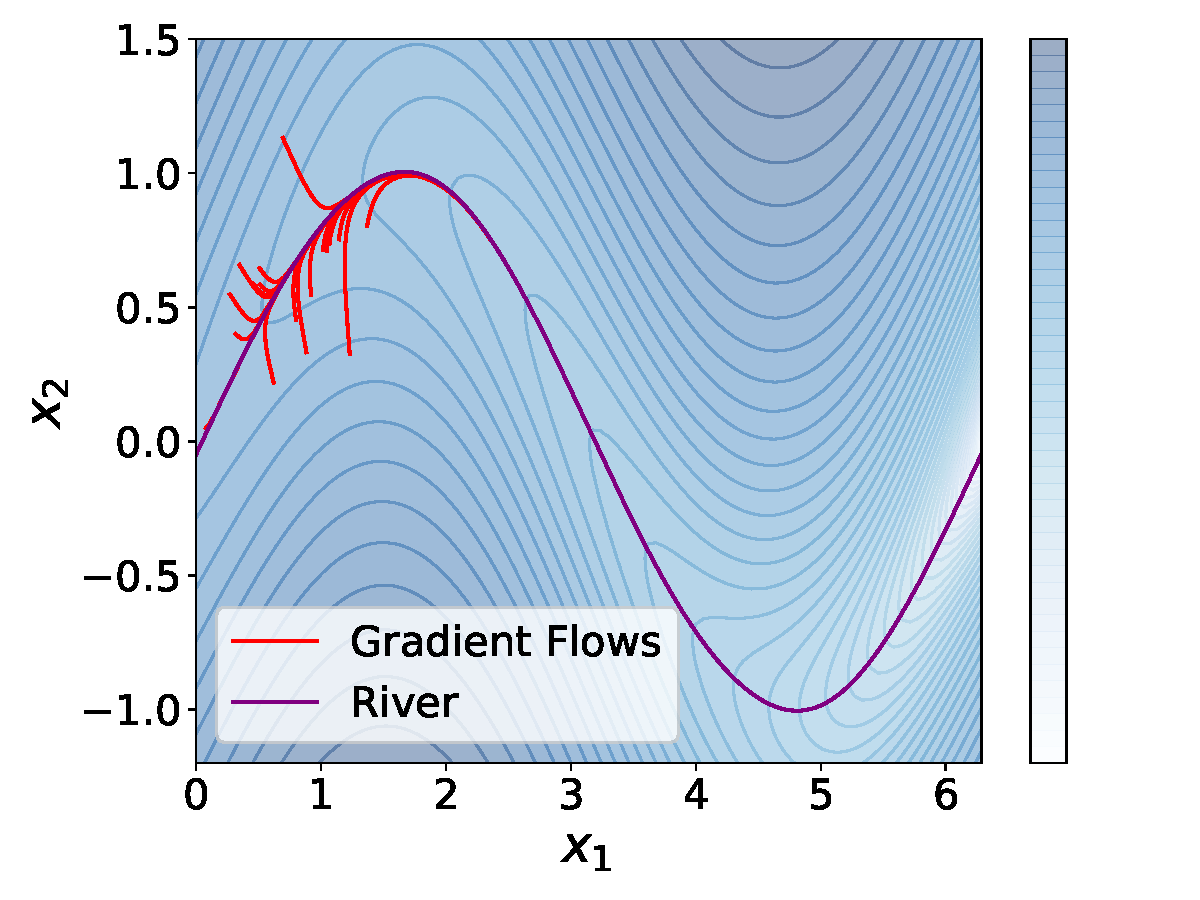
\includegraphics[width=\textwidth]{figures/arxiv/toy_loss_function.pdf}
        \caption{Gradient Flow Dynamics}
        \label{fig:gf}
    \end{subfigure}
    \begin{subfigure}[b]{0.32\textwidth}
        \centering
        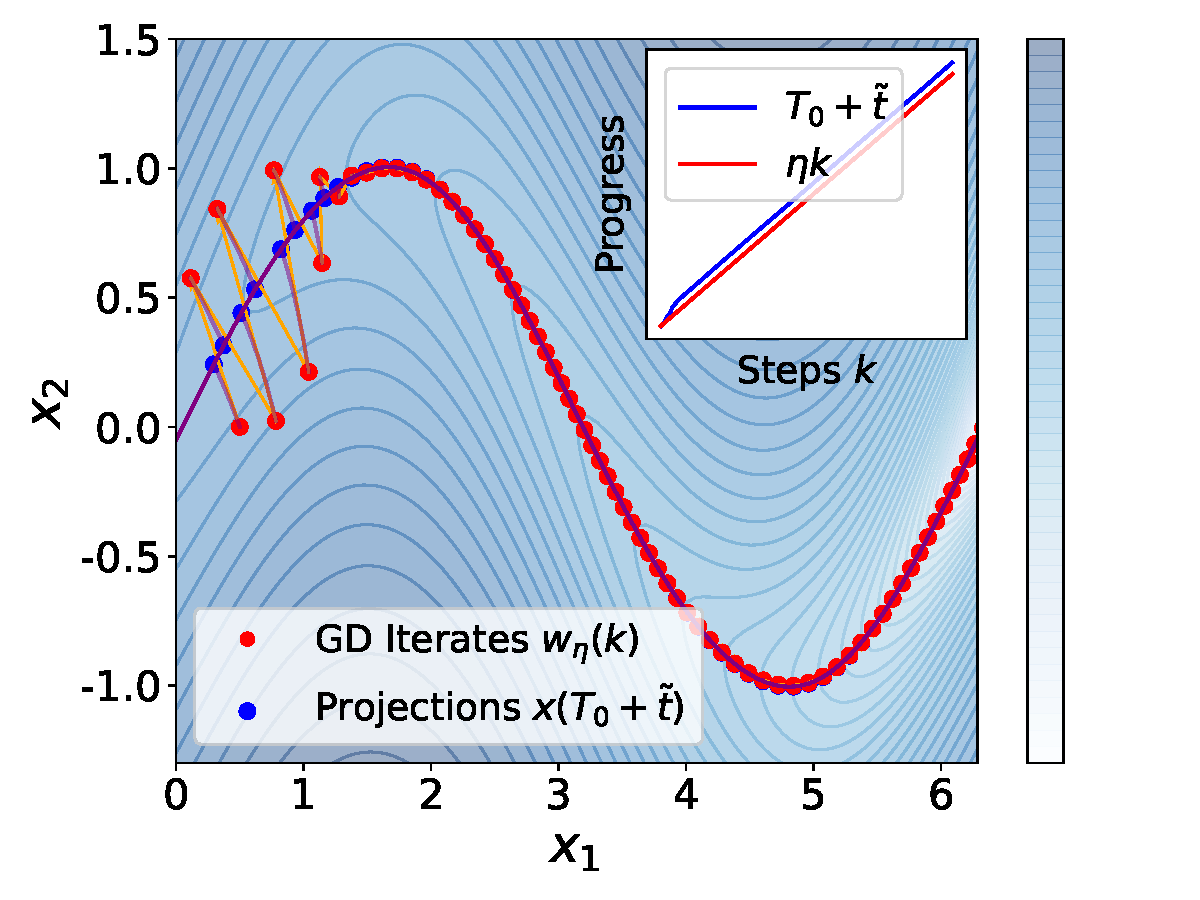
\includegraphics[width=\textwidth]{figures/arxiv/thm2.pdf}
        \caption{Gradient Descent Dynamics}
        \label{fig:gd}
    \end{subfigure}
    \begin{subfigure}[b]{0.33\textwidth}
        \centering
        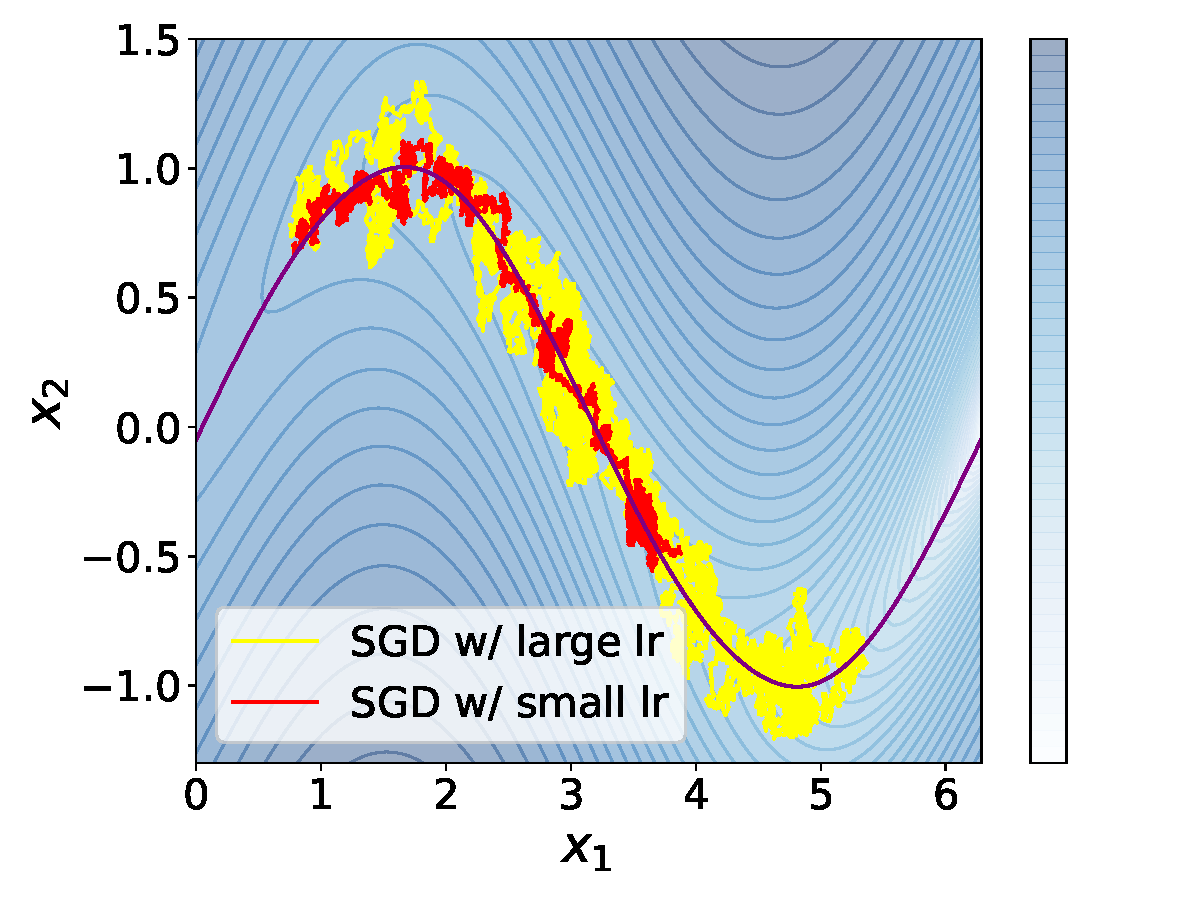
\includegraphics[width=\textwidth]{figures/arxiv/toy_loss_sgd.pdf}
        \caption{Stochastic Gradient Descent}
        \label{fig:sgd}
    \end{subfigure}
        \caption{
                \textbf{Illustration of Theory.} 
         We validate our theory using a 2D example. The \textcolor{blue}{blue curve} represents the "river", where the gradient aligns with the minimal eigenvector of the Hessian. (Left) Randomly initialized \textcolor{red}{gradient flows} converge near the river and follow it closely thereafter. (Middle) Discrete step-size gradient descent shows similar behavior: after initial oscillations, the \textcolor{red}{gradient descent iterates} align closely with their \textcolor{blue}{projections} on the river. (Right) Stochastic gradient descent (SGD) also tracks the river. In contrast to the discrete-step gradient descent, the iterates oscillate around the river rather than staying on it. The {trajectory} with a larger learning rate exhibits faster progress and greater oscillations than {trajectory} with a smaller learning rate.
        }
         \label{fig:toyloss}
        \vspace{-0.2in}
\end{figure}



The proof is deferred to~\Cref{app:gf}. In this theorem, the lower bound on $T$ represents the time required for the iterate to converge near the river. Here $x(T_0 + \tilde{t}) $ can be viewed as a projection of $w(t)$ onto the river. 
As both the geometric error ($2\err\normbound/\gamma$) and the time-alignment error ($\epsilon$) vanish when $\kappa$ is small, this projection is not only close to $w(t) $ but also moves at nearly the same rate as the reference flow. Here the term $T_0$ acts as a shift, reflecting the dependency on the initialization, as optimization trajectories starting from different initial points will enter the river at distinct locations. The term $\tilde t$ represents the progress made along the river. This interpretation will remain consistent in the subsequent sections.

\emph{Proof Sketch.} The proof of \Cref{thm:gftracksriver} relies heavily on the structure of the Hessian matrix. The eigengap assumption (\Cref{assum:technical}.3) ensures that the loss constrained to the mountain dimensions is steep and convex enough to guarantee convergence to the river. The slow spinning assumption (\Cref{assum:technical}.4) ensures that the river direction does not change rapidly, allowing the iterate to follow the river closely after convergence.




\subsection{Gradient Descent Dynamics}


We will now analyze gradient descent with a discrete learning rate. This process is inherently discrete, differentiating it from the continuous gradient flow analyzed above. Similar to the continuous case, an iterate far from the river will converge to the river (as visualized in the first few steps of \Cref{fig:gd}). 
To ease our analysis, we will skip the convergence analysis and assume the starting point $w$ lies on the course of the river. 

\begin{align}
\label{eq:gdflow}
    w_{\eta}(k + 1) - w_{\eta}(k) = - \eta \nabla L(w_{\eta}(k)), \quad w_{\eta}(0) = w \in \river.  
\end{align}

Here we use $k$ to denote the discrete time step, in contrast to the continuous time variable $t$ used in the previous section.
When the learning rate $\eta$ is small, despite the discretization error, gradient descent will still track the river closely at approximately the same pace as the reference flow similar to gradient flow.  In this case, the progress over $k$ steps will be approximately $\eta k$, as shown in the following theorem. 


\begin{theorem}
\label{thm:gdtracksriver}
If a loss $L$ is a river valley (\Cref{def:river-valley}), when $\eta < \frac{\gamma}{2\maxgamma^2}$, for the gradient descent $w_{\eta}(k)$ defined in~\Cref{eq:gdflow} with initialization $w$ on the river, there exists a time shift $T_0$ depending on $w$ and $\eta$, satisfying that for any $\eta k \le \maxT$, there exists a $\tilde t \in [(1-\epsilon)\eta k, (1+\epsilon)\eta k]$  satisfying that,
\begin{align*}
\| x(T_0 + \tilde{t}) - w_{\eta}(k) \|_2 &\le  10 \err \normbound/\gamma\,,
\end{align*}
for $\epsilon = 30 \err + 4\eta \flatgamma$. 
\end{theorem}




The proof is deferred to~\Cref{app:gd}. We observe that the distance of the iterates from the river remains on the same order as in Theorem~\ref{thm:gftracksriver}. However, the learning rate will affect the pace of the iterates, introducing the additional error term $\eta \flatgamma$ in time-alignment error ($\epsilon$). This term is unavoidable, as the discretization inherent in gradient descent introduces a slight deviation from the continuous gradient flow, even in the absence of the hill component of the loss. Finally, the 
\Cref{thm:gdtracksriver} predicts that a larger learning rate $\eta$ will induce higher progress $\eta k$ down the river given the same number of steps $k$. 

We illustrate~\Cref{thm:gdtracksriver} in~\Cref{fig:gd}. Here the {\textcolor{red}{red}} points correspond to gradient descent iterates and {\textcolor[rgb]{0.0, 0.5, 0.0}{green}} points are the corresponding predicted projected points on the river. As the theory predicts, the distance between the iterates and projections diminishes after a few steps. Finally, the inset indicates that the projected points traverse the reference flow on the river at a rate proportional to the learning rate $\eta$.


\subsection{Stochastic Gradient Descent Dynamics}


The above analysis holds for deterministic dynamics and we will now proceed to model the stochasticity in the optimization process. This stochasticity will stop the iterate from fully converging to the river and lead to oscillation in the mountain direction. To simplify the analysis, we will consider a special case where the river direction is a constant and the river reduces to a straight line. We conjecture that the results below can be generalized to a more general setup and leave the detailed analysis to future work.

\begin{assumption}[Straight River]
\label{assum:straight}
For $U$ in~\Cref{assum:technical}, $\forall w \in U, \| \nabla  v_d(\nabla^2 L(w)) \|_2  = 0$. In this case, the river is a straight line parallel to the direction of $v_d(\nabla^2 L(w))$.
\end{assumption}

Under~\Cref{assum:straight}, $v_d(\nabla^2 L(w))$ is a constant vector for $w\in U$ and we will use $v_d$ to denote this vector. We will also assume that the update is deterministic in the direction of the river, which simplifies our proof while still capturing the essential dynamics of SGD. Consequently, we can express the SGD update as follows:
\begin{align}
    \tilde w(k + 1) = \tilde w_k - \eta_k \nabla L\left(\tilde w\left(k\right)\right)  + \eta_k \noise_k, \quad \noise_k \sim \normal{0}{\sigma^2 \left(\identity_d - v_d v_d^T \right)}, \quad \tilde w(0) = w \in \river.  \label{eq:sgd}
\end{align}
Here $\normal{\mu}{\Sigma}$ indicates the normal distribution with mean $\mu$ and covariance $\Sigma$. Compared to deterministic gradient descent, the introduced noise $\noise_k$ causes the iterates to deviate from the river instead of fully converging to it (see the difference between~\Cref{fig:gd} and~\Cref{fig:sgd}). Consequently, we need to impose additional assumptions on the loss landscape to analyze the dynamics of SGD.

\begin{assumption}[Regularity Assumption for SGD]
\label{assum:noise}
In the setting of Assumptions 2, we assume in addition the following:
\begin{enumerate}[leftmargin=*]
    \item {Bounded Hessian.} There exists a constant $\tau > 0$, such that for any weight $w \in U$, the nuclear norm of the Hessian is bounded. 
    $$\| \nabla^2 L(w) \|_{*}  =  \sum\limits_{i = 1}^{d} |\eigen{i}{\nabla^2 L(w)}| \le \tau. $$
    \item {Bounded Third Order Gradient.} There exist  constants $\rho > 0, \kappa' \in [0, 0.01]$, such that,
    \begin{align*}
        \| \nabla^3  L(w) \|_{\textup{op}} \le \rho, \quad \Delta \rho \le \kappa' \gamma^2.
    \end{align*}
    \item {Bounded Loss.} There exists a constant $M > 0$ such that $\forall w, L(w) < M$.
\end{enumerate}
\end{assumption}

In this assumption, we treat $\kappa'$ as a small constant, indicating that the influence of the third-order gradient is minimal. This suggests that the overall shape of the loss landscape is predominantly governed by the first and second-order information. 
We will now analyze the dynamics of SGD in two phases: the stable phase and the decay phase. In both phases, the iterates will track the reference flow with progress linear to the sum of the learning rates. At the same time, the iterates will also incur a loss due to the noise, which will be linear with respect to the learning rate on the last step.



\subsubsection{Stable Phase} 

We start with the stable phase, where the learning rate \(\eta_k = \eta\) remains constant. Similar to the deterministic case, we will demonstrate that the expected loss of the iterate \(\E[L(\tilde{w}(t))]\) closely follows the loss along the reference flow \(L(x(T))\), with \(T \approx \eta t\). However, the stochasticity in the updates introduces an additional term, \(\eta \sigma^2\), into the loss. This provides a formal basis for decomposing the loss into its river and hill components, that is, $L(x(T))$ and $\eta\sigma^2$, respectively.
 

\begin{theorem}
\label{thm:sgd-main}
Suppose a loss $L$ is a river valley (\Cref{def:river-valley}) and satisfies~\Cref{assum:straight,assum:noise}. Then, for any constants $\delta \in (0,1)$, for sufficiently small learning rate $\eta$ depending on the regularity constants, \footnote{Deferred to~\Cref{assum:regular-L} in Appendix.}, there exists a time shift $T_0$ depending on $w$ and $\eta$, the SGD iterates (defined in~\Cref{eq:sgd}) with $\eta_k = \eta$ satisfies that for any integer $k \in [1 /{\eta\gamma}, \maxT / \eta]$, there exists a $\tilde t \in [(1 - \epsilon_{t}) \eta k, (1 + \epsilon_t) \eta k]$ satisfying that,
\begin{align*}
\E[L\left( \tilde w (k)\right)] - L( x( T_0  + \tilde t))& =  {(d - 1) \eta \sigma^2}/{2} + \epsilon_{L} \end{align*}


where $\epsilon_{t} = 4 \eta \flatgamma$ and $|\epsilon_{L}| \le \tau \eta^2  \sigma^2+ \rho (C {d\eta \sigma^2}/{\gamma})^{3/2} + C \kappa' d \eta \sigma^2 +  \delta (2 M + \eta \sigma^2 d) \ll (d - 1) \eta \sigma^2$ with $C = 200 \log(64 \gamma T/\delta)$. 
\end{theorem}

The proof is deferred to~\Cref{app:sgd}. In~\Cref{thm:sgd-main}, the error term in the approximation of the pace of the projection remains the same as in the deterministic case (\Cref{thm:gdtracksriver}). However, the stochasticity introduces an additional hill component $(d - 1)\eta \sigma^2 / 2$ to the expected loss at the iterate. The hill component increases linearly with the learning rate. The error term in loss term $\epsilon_{L}$ can be decomposed into three parts: (1) $ \tau \eta^2  \sigma^2 + \rho (C {\eta \sigma^2}/{\gamma})^{3/2}$ are higher order discretization effects of learning rate $\eta$; (2) $C \kappa' d \eta \sigma^2$ is caused by the change of the Hessian in the valley dimensions and will diminish when $\kappa'$ is small; (3)  $\delta (2M + \eta \sigma^2 d)$ accounts for the small chances that the iterate will escape the neighborhood of the river due to the stochastic updates. While the theorem only considers the case where $v_d$ is a constant vector, we conjecture that the theorem can be extended to a general setting and verify this conjecture on a toy loss (see \Cref{fig:sgd}). 






\subsubsection{Decay Phase} Finally, we will consider the decay phase in training and will show that a proper decaying schedule can reduce the hill component of the loss rapidly. We will first define our decaying schedule, starting from step $k_s = \left\lceil T/\eta \right\rceil$:
\begin{align}
\label{eq:decaylr}
    \eta_k = 
        \frac{\eta}{2 + (k - k_s)\eta \gamma}, \quad  & k_s \le t \le  1.1 k_s.
\end{align}
We choose this schedule to maximize the loss decrease rate on a quadratic function (see~\Cref{app:quadratic}) because we perform quadratic approximations of the loss near the river in our analysis. Our theorem predicts that the hill component of the loss will decrease linearly with the learning rate under this learning rate schedule, consistent with the empirical findings in~\cite{hu2024minicpm}.




\begin{theorem}
\label{thm:decay-main}
Under the setting of~\Cref{thm:sgd-main}, the SGD iterates (defined in~\Cref{eq:sgd}) with the learning rate schedule defined in~\Cref{eq:decaylr} satisfies that for any integer $k \in [k_s, 1.1 k_s]$, there exists a $\tilde t \in [(1 - \epsilon_{t}) T(k), (1 + \epsilon_t) T(k)]$ satisfying that, 
\begin{align*}
\E[L\left( \tilde w (k)\right)] - L( x( T_0 + \tilde t ))& \le  {(d - 1) {\color{red}{ \eta_k}} \sigma^2}/{2} + \epsilon_{L} 
\end{align*}
with $T(k) = T + \sum\limits_{i = k_s}^{k} \eta_{i}$.
\end{theorem}

\begin{wrapfigure}{r}{0.34\textwidth}
    \centering
    \vspace{-0.3in}
    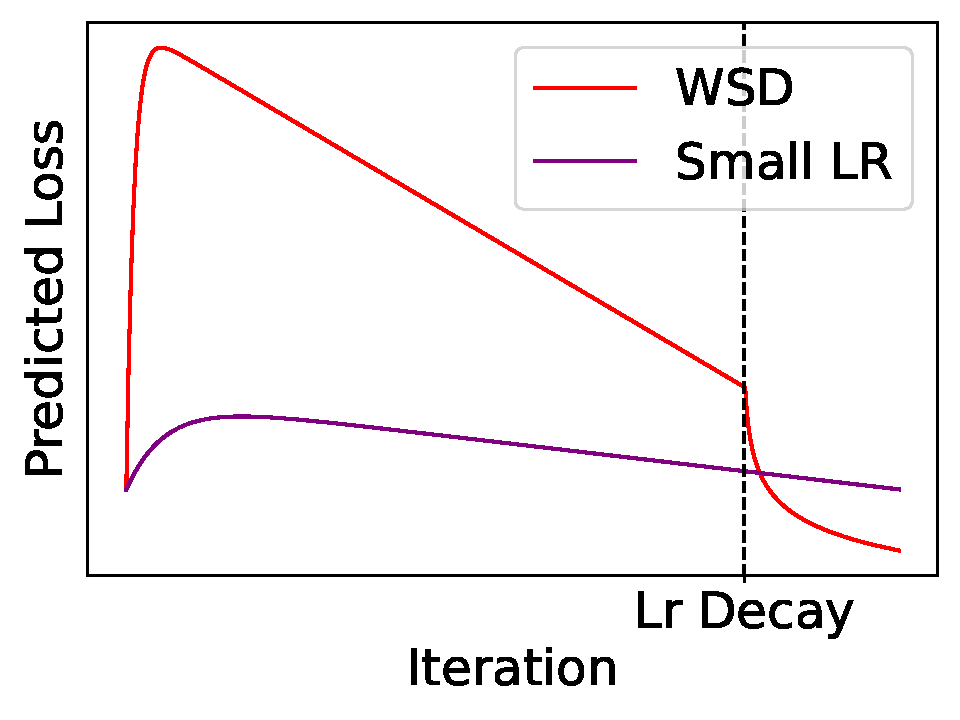
\includegraphics[width=0.3\textwidth]{figures/arxiv/predict.pdf}
    \caption{Predicted Loss Curve of SGD By~\Cref{thm:sgd-main,thm:decay-main} on Loss $L(x_1, x_2) = \gamma x_2^2/2 - x_1$.}
    \label{fig:thmsgd}
    \vspace{-0.4in}
\end{wrapfigure}
The formal proof is deferred to~\Cref{app:decay}. Compared with~\Cref{thm:sgd}, the hill component is now dominated by $(d - 1)\eta_k \sigma^2 / 2$, scaling linearly with the decaying learning rate. 
When the oscillation level $\sigma$ is large compared to the loss changes along the river, the loss decrease can then appear faster in the decay phase than in stable phases (see  \Cref{fig:thmsgd}). Further, the decaying phase also makes progress along the river, which corresponds to the term $\sum\limits_{i = k_s}^k \eta_i$ in the theorem. Finally, the terms used in our theorem match the scaling law formulation in the concurrent work~\citep{tissue2024scalinglawlearningrate}.

\subsection{Future Extensions}
We only consider a 1-dimensional river in the theoretical analysis above. However, it is possible to extend our assumptions to a generalized $k$-dimensional river, where the gradient lies in the flattest $k$-dimensional subspace for every point on the river.

\begin{assumption}
\label{assum:gen-river}
    We assume the existence of a ``generalized river'', which is a $p$-dimensional manifold $\river$ such that any point $w \in \river$ has a gradient $\nabla L(w)$ lies in the eigenspace spanned by the last $k$ eigenvectors' direction of the Hessian, $\{ \eigenv{i}{\nabla^2 L(w)} \mid i \in [d - p + 1, d] \}$. 
\end{assumption}

Based on this assumption, we can define \emph{generalized river valley Structure}. We believe that under some appropriate assumptions, there will be a similar coupling between the dynamics in the original river valley landscape and the dynamics constrained on the generalized river, and leave this for future work.

There are several other potential technical improvements to our theory that could be explored in future works. First, the analysis of the stochastic setting may be extended to include a river that is not a straight line. Second, the multiplicative constant of 4 in the eigengap condition (Assumption 2.3) might be eliminated through more refined analysis. Lastly, the upper bound on the learning rate in~\Cref{thm:gdtracksriver} (currently $\gamma / 2\maxgamma^2$) could potentially be improved to $\Theta(1/ \maxgamma)$ through more fine-grained analysis, which is the maximal learning rate in the quadratic case.

\subsection{Visualizing the River Valley} 
We use a direct probing method to verify our theory. Our theory suggests that when the learning rate is large, the model will bounce back and forth between the sharp valleys. However, in the decay phase, the model will move downwards the hillside to approach the river. This suggests that if we connect two checkpoints in the stable phase, we should expect to see a projection of the valley, and if we connect two checkpoints in the decay phase, we should expect to see smooth decreasing curves. To verify this, we pretrain a 124M GPT-2 model on OpenWebText. In the first run, we train the model with a constant learning rate for 25B tokens and interpolate between two checkpoints at 20B and 25B tokens (\Cref{fig:highconnect}). In the second run, we branch off from the first run at 20B tokens and decay the learning rate for 5B tokens, and we interpolate between two checkpoints at 20B and 25B tokens (\Cref{fig:rampconnect}).
The interpolation results closely resembles our theory. This observation is also consistent with~\cite{sanyal2023early} which shows weight averaging improves model performance in the earlier part of the cosine training runs, where the learning rates are higher. Additionally, the smooth decreasing curves we observed when connecting two checkpoints in the decay phase are consistent with the findings in~\cite{hagele2024scalinglawscomputeoptimaltraining}.
\begin{figure}[t]
    \centering
    \begin{subfigure}[b]{0.30\textwidth}
        \centering
        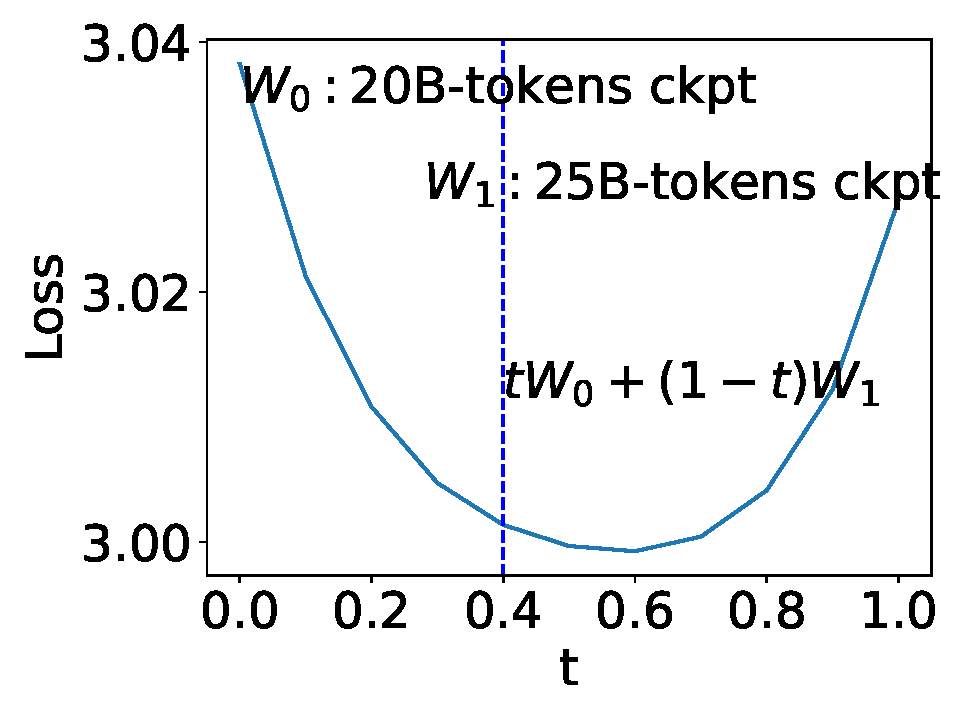
\includegraphics[width=\textwidth]{figures/arxiv/highway_interp_new.pdf}
        \caption{Stable Phase}
        \label{fig:highconnect}
    \end{subfigure}
    \begin{subfigure}[b]{0.30\textwidth}
        \centering
        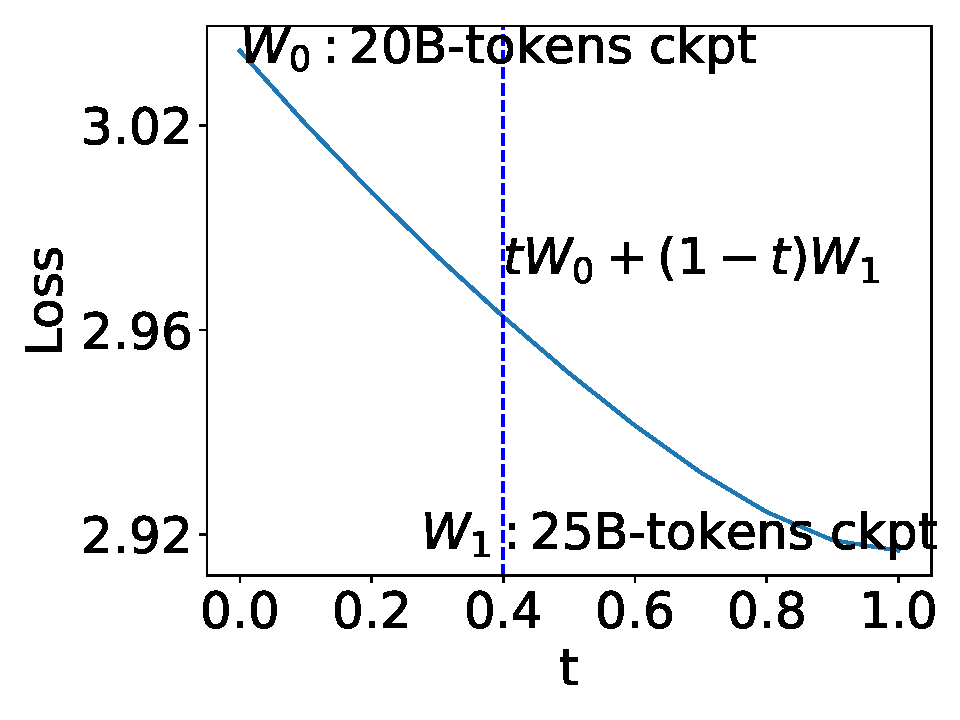
\includegraphics[width=\textwidth]{figures/arxiv/ramp_interp_new.pdf}
        \caption{Decay Phase}
        \label{fig:rampconnect}
    \end{subfigure}
    \quad
    \begin{minipage}[b]{0.36\textwidth}%
        \caption{\textbf{Probing Loss Landscape.}  We validate the river valley analogy by interpolating stable and decay phases in GPT-2 pretraining experiments. We observe that loss resembles a valley when constrained on the segment connecting two models during the stable phase and smoothly decreases when connecting two models during the decay phase.}
        \label{fig:loss}
    \end{minipage}
\end{figure}






